\documentclass[conference]{IEEEtran}
\IEEEoverridecommandlockouts
% ---------------------------------------------------------------------------
% Packages
% ---------------------------------------------------------------------------
\usepackage{cite}
\usepackage{amsmath,amssymb,amsfonts}
\usepackage{algorithmic}
\usepackage{graphicx}
\usepackage{textcomp}
\usepackage{xcolor}
\usepackage{hyperref}
\usepackage{booktabs}
\usepackage{tikz}
\usetikzlibrary{arrows.meta, positioning, shapes.geometric, fit, backgrounds}
\usepackage{listings}
\usepackage{caption}
\usepackage{subcaption}

\lstset{
  basicstyle=\ttfamily\footnotesize,
  breaklines=true,
  columns=fullflexible,
  frame=single,
  numbers=left,
  numberstyle=\tiny,
  captionpos=b
}

\def\BibTeX{{\rm B\kern-.05em{\sc i\kern-.025em b}\kern-.08em
    T\kern-.1667em\lower.7ex\hbox{E}\kern-.125emX}}

% ---------------------------------------------------------------------------
\begin{document}

\title{Sentinel: A Client-Side Browser Extension for\\Real-Time Phishing Detection}

\author{
\IEEEauthorblockN{Shawn}
\IEEEauthorblockA{
Independent Project \\
Email: shawngeorge530@gmail.com}
}

\maketitle

\begin{abstract}
Phishing remains one of the most persistent and cost-effective attack vectors on the web, relying on convincing but fraudulent pages that imitate legitimate login and payment flows. Server-side and blocklist-based defenses are reactive by construction: a page must be reported, crawled, and classified before it is blocked, leaving a window in which new or short-lived phishing campaigns succeed. This report describes Sentinel, a client-side browser extension that scores pages for phishing risk in real time, in the browser, without depending on a remote classification service for every page view. We describe the problem space, the design rationale for a heuristic-plus-learned-features scoring engine compiled to WebAssembly, the implementation across the extension, scoring engine, and offline data/evaluation pipeline, and a multi-pronged evaluation plan spanning fixture-corpus regression testing, usability testing with real participants, and comparison against existing anti-phishing approaches.
\end{abstract}

\begin{IEEEkeywords}
phishing detection, browser extension, client-side security, WebAssembly, usable security
\end{IEEEkeywords}

% =============================================================================
\section{Introduction}
% =============================================================================
Phishing attacks continue to be a dominant initial-access technique in both consumer and enterprise breaches. Attackers exploit the visual and structural similarity between a fraudulent page and its legitimate counterpart, relying on a victim's fast, low-scrutiny judgment of a familiar-looking login form. Existing defenses largely operate at the network or reputation layer: DNS/URL blocklists, browser-vendor Safe Browsing style services, and email-gateway filtering. These approaches are effective at scale but are inherently reactive --- a URL typically must be observed, reported, and propagated to a blocklist before protection takes effect, and short-lived or newly-registered phishing domains can operate for hours before they are listed.

This project, Sentinel, takes a complementary, client-side approach: rather than relying solely on a maintained blocklist, the extension inspects the structure and content of the page the user is actually viewing --- its DOM, form fields, and brand-impersonation signals --- and produces a real-time risk score entirely in the browser. This report documents the motivation, design, implementation, and evaluation strategy for the system.

% =============================================================================
\section{The Problem}
% =============================================================================
Phishing detection systems face several concrete, competing constraints:

\begin{itemize}
  \item \textbf{Reaction latency.} Blocklist-based protection cannot cover a domain until it has already been observed and classified, which is systematically too slow for campaigns that live for only a few hours.
  \item \textbf{Privacy and trust.} Sending every visited URL or page content to a remote classification service raises privacy concerns and introduces a dependency that itself becomes a target and a single point of failure.
  \item \textbf{False positives erode trust.} An overly aggressive detector that flags legitimate login pages trains users to dismiss warnings, which is worse than no warning at all --- this is a usability problem as much as a detection-accuracy problem.
  \item \textbf{Explainability.} A binary "blocked/not blocked" signal gives the user no way to evaluate the warning; without an explanation, users cannot build calibrated trust in the tool.
  \item \textbf{Evolving adversary.} Attackers adapt to detection heuristics (e.g., cloaking, dynamic DOM injection), so any static rule set decays over time and must be continually re-evaluated against fresh data.
\end{itemize}

The problem, therefore, is not simply "classify a page as phishing or not," but to do so \emph{client-side}, \emph{in real time}, \emph{with an explanation}, and in a way whose accuracy can be \emph{continuously measured and regression-tested} as both the page corpus and the detection logic evolve.

% =============================================================================
\section{Proposed Solution}
% =============================================================================
Sentinel addresses this with a three-part system:

\begin{enumerate}
  \item \textbf{A Manifest V3 Chrome extension} that runs a content script on every page load, extracts a feature vector from the live DOM (form structure, credential-field detection, brand/logo signals, URL structure, TLS/host anomalies), and displays a color-coded badge (green/amber/red) together with a popup explanation.
  \item \textbf{A shared scoring engine, written in Rust and compiled to WebAssembly}, so that the same scoring logic can run deterministically both inside the browser (for real-time scoring) and inside the offline Python evaluation pipeline (for regression testing against a frozen corpus), eliminating train/serve skew between "what we evaluate" and "what ships."
  \item \textbf{An offline data and evaluation pipeline} (Python, \texttt{uv}-managed) that collects and curates benign and phishing samples, maintains a frozen fixture corpus and dataset manifest for reproducible evaluation, and gates continuous integration on a recall/false-positive-rate threshold so that changes to the heuristics cannot silently regress detection quality.
\end{enumerate}

This design deliberately favors a transparent, inspectable heuristic-plus-features engine over an opaque server-side ML classifier for the initial version, in order to keep scoring local, auditable, and explainable to the end user, while leaving room to introduce a trained model (e.g., LightGBM) on top of the same feature pipeline once sufficient labeled data is frozen.

% =============================================================================
\section{Related Work}
% =============================================================================
Prior anti-phishing approaches broadly fall into several categories:

\textbf{Blocklist/reputation services} (e.g., Google Safe Browsing, Microsoft SmartScreen) maintain centrally curated lists of known-malicious URLs, propagated to browsers. They are highly precise but latent, offering no protection against domains that have not yet been crawled and classified.

\textbf{Visual-similarity detection} approaches compare a suspected page's rendered appearance or screenshot against a reference set of legitimate brand pages (e.g., logo and layout matching) to detect impersonation, at the cost of requiring a maintained reference-brand database and being comparatively expensive to run per page view.

\textbf{URL-lexical and host-based classifiers} use statistical/ML features of the URL string and host metadata (domain age, WHOIS data, character n-grams, Tranco/popularity rank) to flag suspicious links; these are lightweight but blind to page content and can be defeated by long-lived, legitimately-registered infrastructure used for a short phishing campaign.

\textbf{DOM/content-based heuristic classifiers} inspect the structure of the page itself --- form actions, password-field targets, favicon/brand mismatches --- which is the closest category to this project's approach, and which several academic and open-source anti-phishing toolbars have explored, generally trading off explainability against raw model accuracy.

Sentinel's contribution relative to this landscape is architectural rather than a novel detection algorithm: it packages DOM/content heuristics and a Tranco-popularity/bloom-filter brand check into a single WebAssembly engine shared verbatim between the live extension and an offline, CI-gated evaluation harness, and treats the usability of the warning (explanation quality, click-through rate on true warnings) as a first-class, measured requirement rather than an afterthought.

% =============================================================================
\section{Software Design Considerations}
% =============================================================================
\subsection{Design Goals}
From first principles, four goals drove the architecture:
\begin{enumerate}
  \item \textbf{No server dependency for scoring.} Every page-load decision must be computable locally, so scoring cannot introduce added latency, an external outage, or a privacy leak of visited URLs.
  \item \textbf{One source of truth for scoring logic.} The exact code that scores a page in the browser must be the same code exercised by the offline evaluation suite, or accuracy numbers measured offline would not reflect what ships.
  \item \textbf{Reproducible, regression-tested accuracy.} As heuristics change, detection quality must be measurable against a frozen, version-controlled corpus, not just "look right" in ad hoc manual testing.
  \item \textbf{Explainable output.} The extension should be able to say \emph{why} a page was scored the way it was, not only emit a score.
  \end{enumerate}

\subsection{Architecture Overview}
These goals motivate a layered architecture (Fig.~\ref{fig:architecture}): a thin browser-integration layer (content/background/popup scripts) sits on top of a portable feature-extraction and scoring core compiled once to WebAssembly and consumed both by the extension bundle and by the Python evaluation harness through the same compiled artifact family.

\begin{figure}[t]
\centering
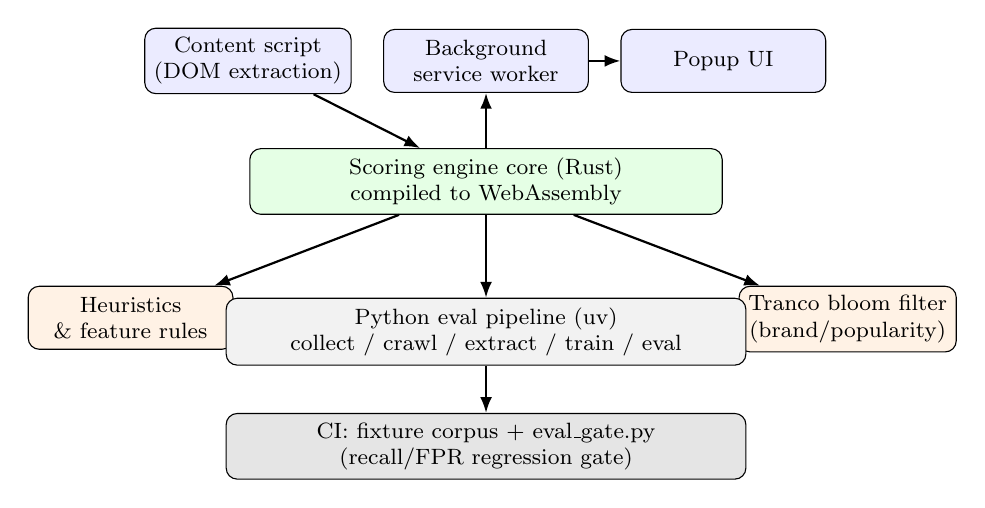
\begin{tikzpicture}[
  box/.style={draw, rounded corners, minimum width=2.6cm, minimum height=0.8cm, align=center, font=\footnotesize},
  arr/.style={-{Latex[length=2mm]}, thick}
]
\node[box, fill=blue!8] (content) {Content script\\(DOM extraction)};
\node[box, fill=blue!8, right=0.4cm of content] (bg) {Background\\service worker};
\node[box, fill=blue!8, right=0.4cm of bg] (popup) {Popup UI};

\node[box, fill=green!10, below=0.7cm of bg, minimum width=6cm] (engine) {Scoring engine core (Rust)\\compiled to WebAssembly};

\node[box, fill=orange!10, below left=0.9cm and 0.2cm of engine] (heur) {Heuristics\\\& feature rules};
\node[box, fill=orange!10, below right=0.9cm and 0.2cm of engine] (bloom) {Tranco bloom filter\\(brand/popularity)};

\node[box, fill=gray!10, below=2.6cm of bg, minimum width=6.6cm] (pipeline) {Python eval pipeline (uv)\\collect / crawl / extract / train / eval};

\node[box, fill=gray!20, below=0.6cm of pipeline, minimum width=6.6cm] (ci) {CI: fixture corpus + eval\_gate.py\\(recall/FPR regression gate)};

\draw[arr] (content) -- (engine);
\draw[arr] (engine) -- (bg);
\draw[arr] (bg) -- (popup);
\draw[arr] (engine) -- (heur);
\draw[arr] (engine) -- (bloom);
\draw[arr] (engine.south) -- (pipeline.north);
\draw[arr] (pipeline) -- (ci);
\end{tikzpicture}
\caption{Sentinel architecture: a shared WebAssembly scoring core is consumed by the browser extension for live scoring and by the Python pipeline for offline, CI-gated evaluation, avoiding train/serve skew.}
\label{fig:architecture}
\end{figure}

\subsection{Key Design Decisions}
\begin{itemize}
  \item \textbf{Rust/WebAssembly over pure JavaScript for the engine.} Compiling the scoring core once and consuming it from both TypeScript (extension) and Python (pipeline, via the same compiled artifact / equivalent scoring path) removes duplicated logic that would otherwise drift between "what we evaluate offline" and "what actually ships," which was judged a higher risk than the added build complexity of a Rust toolchain.
  \item \textbf{Manifest V3 over V2.} MV3's service-worker background model is required for current and future Chrome Web Store submissions; the design accepts MV3's more restrictive persistent-state model (no long-lived background page) in exchange for store compliance and longevity.
  \item \textbf{Heuristics-first, model-ready pipeline.} Rather than shipping an opaque classifier from day one, the initial version scores with inspectable heuristics and feature rules, while the pipeline's \texttt{train}/\texttt{export} stages are already structured to plug in a trained model (e.g., LightGBM) once the frozen dataset is large enough, without changing the extension-side interface.
  \item \textbf{Frozen, hashed fixture corpus for CI.} Real crawled phishing/benign data is privacy- and licensing-sensitive and is kept local (gitignored); a synthetic, hash-manifested fixture corpus is committed instead, so CI evaluation is reproducible without redistributing sensitive crawl data.
  \item \textbf{Bloom filter for brand/popularity lookups.} A Tranco-derived Bloom filter gives a compact, constant-size, false-positive-bounded structure for "is this a known-popular domain" checks inside the extension bundle, avoiding shipping a full domain list.
\end{itemize}

% =============================================================================
\section{Implementation}
% =============================================================================
\subsection{How the System Works End to End}
On each page load, the content script extracts a feature vector from the live DOM (form actions and input types, presence of password fields, external resource origins, brand/logo heuristics, and URL structure). This feature vector is passed to the WebAssembly scoring engine, which returns a risk score and a set of contributing signals. The background service worker receives the score, sets the toolbar badge color (green/amber/red), and stores per-tab state; the popup queries this state to render a human-readable explanation and exposes a "Trust this site" allowlist action.

\subsection{Deployment}
The extension is built with Vite and the \texttt{@crxjs/vite-plugin}, which compiles TypeScript sources and generates the MV3 \texttt{manifest.json} into a distributable \texttt{dist/} directory. For local/manual testing this directory is loaded directly via Chrome's \emph{Load unpacked} developer flow; for distribution to testers it is additionally zipped into a versioned artifact (e.g., \texttt{sentinel-0.1.0.zip}) suitable for sideloading or, ultimately, Chrome Web Store submission.

\subsection{Nitty-Gritty Implementation Details}
\begin{itemize}
  \item The workspace is a \texttt{pnpm} monorepo with separate packages for the extension application, the feature-extraction library, the heuristics library, and the Rust-based WebAssembly engine, each independently unit-tested.
  \item The Rust engine is compiled with \texttt{wasm-pack} targeting \texttt{web}, producing a JS-consumable WASM module (\texttt{sentinel\_engine}) shared between the extension bundle and equivalent scoring logic exercised from the Python side for evaluation.
  \item Bundle size is actively budgeted and enforced (a size-limit configuration fails the build if the extension bundle exceeds its budget), since content-script payload size directly affects page-load overhead on every site the user visits.
  \item The Python side is dependency-locked and managed with \texttt{uv}, with distinct pipeline stages for \texttt{collect} (curated benign/phishing sample collection), \texttt{crawl}, \texttt{extract} (feature extraction matching the client-side extractor), \texttt{train}, \texttt{export}, and \texttt{eval}.
\end{itemize}

\subsection{User Interface}
The UI surface is intentionally minimal: a toolbar badge communicates risk at a glance without requiring interaction, and the popup (opened on click) shows the score, a short natural-language explanation of \emph{why} the page was flagged, and a single primary action to allowlist a trusted site. This minimal-friction design is a direct response to the usability constraint in Section~\ref{sec:eval}: warnings that require multiple clicks or dense text to parse are more likely to be dismissed unread.

\subsection{Integration and Testing}
The project integrates three toolchains under one CI pipeline (Fig.~\ref{fig:architecture}, bottom):
\begin{itemize}
  \item \textbf{TypeScript/extension layer:} \texttt{vitest} unit tests per package, plus a combined \texttt{format:check + typecheck + lint + test:coverage} gate.
  \item \textbf{Rust/WASM layer:} \texttt{cargo test --workspace}, plus a WASM build step that must succeed.
  \item \textbf{Python pipeline layer:} \texttt{ruff} linting and \texttt{pytest} covering the Bloom filter, curated-benign filtering, dataset freezing, metrics computation, and storage logic.
  \item \textbf{End-to-end layer:} Playwright drives the \emph{actual built extension} in headless Chromium against a fixture-page corpus, verifying the full content-script $\rightarrow$ engine $\rightarrow$ badge/popup path rather than any single unit in isolation.
  \item \textbf{Detection regression gate:} the offline evaluation harness scores a frozen fixture corpus and an automated gate script fails the build if recall or false-positive rate at the ``medium'' risk threshold regresses past a fixed bound, preventing heuristic changes from silently degrading accuracy.
\end{itemize}

% =============================================================================
\section{Evaluation}
\label{sec:eval}
% =============================================================================
Evaluating a phishing detector requires more than a single accuracy number, because the system has two different audiences with different failure costs: the end user (who is harmed by a missed detection or annoyed by a false alarm) and the security community (who compares it against existing tools). This project's evaluation plan is organized along four axes.

\subsection{Evaluation by External Users}
A structured usability protocol runs a small cohort (5--10 participants) through four representative tasks: judging a high-risk fixture page, explaining what a warning score means in their own words, allowlisting a medium-risk fixture, and using the popup to check an arbitrary link. Metrics collected include an explanation-comprehension score, time-to-decision, allowlist discoverability, and a 1--5 trust/annoyance rating; critically, the click-through rate on true high-risk warnings is treated as a hard release blocker above a fixed threshold, since a warning nobody heeds provides no real protection regardless of underlying detection accuracy.

At the time of writing, the full multi-participant study has not yet been run. As a first, real (non-hypothetical) data point, a single-session pilot walkthrough of the built extension was carried out against the live fixture corpus, exercising the same four tasks; full results are recorded in \texttt{docs/usability-pilot-ai-walkthrough.md} and summarized here with the explicit caveat that $n=1$ and the session was tool-automated rather than run with a human participant, so no claim from it generalizes.

On the high-risk \texttt{ip-login} fixture, the extension did not wait for user interaction: it blocked the page within roughly two seconds of load with a full-screen interstitial (``Stop --- this page is probably phishing'') that named the specific triggering signals (raw-IP host, password field on an insecure connection, a login form injected after page load) rather than a generic warning. Scored against the protocol's 0--2 explanation rubric, this reached 2/2. Attempting to click through surfaced a \emph{second}, independent confirmation dialog (``Passwords typed here may be stolen. Continue?'') before the page became usable --- a stronger friction pattern than the single-warning model the $\leq$15\% click-through target assumes, and a point in the design's favor. The allowlist action (``This site is safe'') was directly visible on the resulting persistent banner with no need to open a separate popup, was reachable in one click without prior guidance, and was confirmed to persist correctly across a page reload. One benign fixture (\texttt{bank-login}) produced no false warning.

One discrepancy surfaced that warrants follow-up before being cited as a settled result: the \texttt{http-login} fixture, whose offline score (Section~VI-B) places it at the MEDIUM threshold, triggered the same blocking interstitial as the HIGH-risk case in this pilot rather than a lighter-weight treatment. This may be an artifact of the pilot accessing fixtures via \texttt{localhost} rather than their designed hostnames (losing a hostname-based scoring signal shifts the total score), or it may reflect that the current build does not yet visually differentiate MEDIUM from HIGH warnings --- the pilot write-up flags this explicitly as needing verification against the intended hostnames rather than asserting either explanation. The pilot also could not exercise the toolbar badge or the popup's ``check a link'' task (T4), since the available automation could reach in-page content but not the browser toolbar or extension-popup surface; those remain untested pending either a human tester or Playwright-based extension automation (as already used in \texttt{tests/e2e/}).

\subsection{Evaluation Against Similar Systems}
The system can be benchmarked against three categories of comparison baseline drawn directly from Section~IV: (1) blocklist/reputation-only protection (e.g., browser-native Safe Browsing-style blocking), measured on time-to-protection for newly-registered domains; (2) URL-lexical classifiers, measured on precision/recall using the same frozen corpus; and (3) other open-source DOM/content-heuristic extensions, measured on both detection metrics and bundle/runtime overhead. Comparable metrics --- recall and false-positive rate at a fixed operating threshold, using the project's own \texttt{run\_eval.py}/\texttt{eval\_gate.py} scoring path --- allow an apples-to-apples comparison once equivalent datasets are run through each system.

As a baseline against which future comparisons can be measured, running \texttt{pnpm evaluate} against the current 20-row fixture corpus (10 phishing, 10 benign, from \texttt{docs/eval-results.json}) yields ROC AUC~$=1.0$ and PR~AUC~$=1.0$; at the MEDIUM decision threshold, precision, recall, and F1 are all $1.0$ (0 false positives, 0 false negatives); at the HIGH threshold, precision remains $1.0$ but recall drops to $0.9$ (one phishing case, \texttt{http-login}, scores only into the MEDIUM band rather than HIGH). These numbers should be read as an internal regression baseline on a small, synthetic, team-authored corpus rather than a competitive accuracy claim --- the comparison against external baselines described above has not yet been run, and Section VI-C explains why the sample size limits confidence in the figures themselves.

\subsection{Limitations Relative to Other Systems}
\begin{itemize}
  \item The current heuristic engine has no trained ML component yet (no model artifact is committed), so its ceiling on precision/recall is bounded by hand-authored rules relative to systems using large-scale trained classifiers.
  \item The frozen fixture corpus (on the order of tens of synthetic pages) is far smaller than the crawled corpora typically used to evaluate production anti-phishing systems, limiting the statistical confidence of any accuracy claim until the larger, hashed real-data manifest is frozen and used.
  \item Detection is scoped to page structure/content and known-popularity signals; it does not currently incorporate network-layer signals (TLS certificate transparency, domain age/WHOIS, hosting reputation) that some competing systems use.
  \item As a purely client-side, per-page-load system, it cannot benefit from cross-user telemetry (e.g., "N other users just saw this exact domain") the way centralized reputation services can.
\end{itemize}

\subsection{Directions for Expansion}
The pipeline's \texttt{train}/\texttt{export} stages are already structured to accept a trained model over the existing feature vector, which would let the system move from heuristic scoring to a hybrid heuristic+ML score without changing the extension-side interface. Expanding the frozen dataset (more benign diversity, adversarially-collected phishing kits) would tighten the confidence interval on measured recall/FPR. Longer term, incorporating host/network-layer signals and cross-referencing against public blocklists as an additional, non-blocking signal would let Sentinel combine the low-latency benefit of local scoring with some of the precision benefit of centralized reputation systems.

% =============================================================================
\section{Conclusion and Future Work}
% =============================================================================
Sentinel demonstrates that client-side, real-time phishing detection is practical without depending on a remote classification service for every page view, by compiling a single scoring engine to WebAssembly and sharing it between a browser extension and a CI-gated offline evaluation pipeline. This architecture keeps live scoring auditable and explainable while giving the project a reproducible way to measure whether changes to its detection logic help or hurt, rather than relying on manual spot-checking. The evaluation plan in Section~\ref{sec:eval} treats usability --- specifically, whether real warnings are heeded --- as equally important as raw detection accuracy, reflecting the reality that an ignored warning provides no protection.

Future work includes: freezing and incorporating the larger real-data corpus described in the project's dataset manifest; training and shipping the first learned model on top of the existing feature pipeline; running the usability study with a real participant cohort and iterating on warning copy/UI based on the results; and benchmarking against at least one blocklist-based and one ML-based baseline on a shared dataset to produce a defensible comparative accuracy claim.

% =============================================================================
\section*{Acknowledgment}
% =============================================================================
The author thanks contributors and testers who provided feedback during development.

% =============================================================================
\begin{thebibliography}{00}
% =============================================================================
\bibitem{apwg} Anti-Phishing Working Group, ``Phishing Activity Trends Report,'' APWG, [Online]. Available: https://apwg.org/trendsreports/
\bibitem{safebrowsing} Google, ``Safe Browsing,'' Google Safe Browsing Documentation. [Online]. Available: https://safebrowsing.google.com/
\bibitem{tranco} V. Le Pochat, T. Van Goethem, S. Tajalizadehkhoob, M. Korczy{\'n}ski, and W. Joosen, ``Tranco: A Research-Oriented Top Sites Ranking Hardened Against Manipulation,'' in \emph{Proc. Network and Distributed System Security Symposium (NDSS)}, 2019.
\bibitem{visualsim} Y. Zhang, J. I. Hong, and L. F. Cranor, ``CANTINA: A Content-Based Approach to Detecting Phishing Web Sites,'' in \emph{Proc. 16th International Conference on World Wide Web (WWW)}, 2007, pp. 639--648.
\bibitem{mv3} Google, ``Chrome Extensions: Manifest V3,'' Chrome for Developers. [Online]. Available: https://developer.chrome.com/docs/extensions/mv3/intro/
\bibitem{wasm} A. Haas et al., ``Bringing the Web up to Speed with WebAssembly,'' in \emph{Proc. 38th ACM SIGPLAN Conference on Programming Language Design and Implementation (PLDI)}, 2017.
\bibitem{lightgbm} G. Ke et al., ``LightGBM: A Highly Efficient Gradient Boosting Decision Tree,'' in \emph{Advances in Neural Information Processing Systems (NeurIPS)}, 2017.
\bibitem{bloomfilter} B. H. Bloom, ``Space/Time Trade-offs in Hash Coding with Allowable Errors,'' \emph{Communications of the ACM}, vol. 13, no. 7, pp. 422--426, 1970.
\end{thebibliography}

\end{document}
